\documentclass[a4paper,10pt,twoside]{article}

\usepackage[top=1in, bottom=1in, left=1in, right=1in]{geometry}
\usepackage[utf8]{inputenc}
\usepackage[spanish,es-ucroman,es-noquoting]{babel}
\usepackage{setspace}
\usepackage{fancyhdr}
\usepackage{lastpage}
\usepackage{amsmath}
\usepackage{amsfonts}
\usepackage{verbatim}
\usepackage{graphicx}
\usepackage{float}
\usepackage{algorithmic}
\usepackage{tikz}
\usepackage{ gensymb }
\usetikzlibrary{calc}
\usetikzlibrary{decorations.pathreplacing}


% Evita que el documento se estire verticalmente para ocupar
% el espacio vacío en cada página.
\raggedbottom


%%%%%%%%%% Configuración de Fancyhdr - Inicio %%%%%%%%%%
\pagestyle{fancy}
\thispagestyle{fancy}
\lhead{RTP2, Organización del Computador II}
\renewcommand{\footrulewidth}{0.4pt}
\cfoot{\thepage /\pageref{LastPage}}

\fancypagestyle{caratula} {
   \fancyhf{}
   \cfoot{\thepage /\pageref{LastPage}}
   \renewcommand{\headrulewidth}{0pt}
   \renewcommand{\footrulewidth}{0pt}
}
%%%%%%%%%% Configuración de Fancyhdr - Fin %%%%%%%%%%


%%%%%%%%%% Configuración de Algorithmic - Inicio %%%%%%%%%%
% Entorno propio para customizar la presentación del pseudocódigo
\newenvironment{pseudocodigo}
    {\vspace{0.5em} \begin{algorithmic}}
    {\end{algorithmic} \vspace{0.5em}}

% Alinear comentarios a la derecha
\renewcommand{\algorithmiccomment}[1]{\hfill \{#1\}}
%%%%%%%%%% Configuración de Algorithmic - Fin %%%%%%%%%%


%%%%%%%%%% Macros de tikz - Inicio %%%%%%%%%%
% Uso: \registroCuatro{etiqueta}{x}{y}{a4}{a3}{a2}{a1}
\newcommand{\registroCuatro}[7]{
    \ifthenelse{\equal{#1}{}}{}{
        \draw (#2, {#3 + 0.5}) node[anchor=east]{#1};
    }

    \draw   (#2, #3) rectangle +(4, 1) +(2, 0.5) node{#4}
          ++(4, 0)   rectangle +(4, 1) +(2, 0.5) node{#5}
          ++(4, 0)   rectangle +(4, 1) +(2, 0.5) node{#6}
          ++(4, 0)   rectangle +(4, 1) +(2, 0.5) node{#7};          
}

% Uso: \registroOcho{etiqueta}{x}{y}{a8}{a7}{a6}...{a1}
\newcommand{\registroOcho}[9]{
    \def\etiqueta{#1}
    \def\x{#2}
    \def\y{#3}
    \def\aviii{#4}
    \def\avii{#5}
    \def\avi{#6}
    \def\av{#7}
    \def\aiv{#8}
    \def\aiii{#9}
    \registroOchoX    
}
\newcommand{\registroOchoX}[2]{ % Auxiliar - no usar directamente
    \def\aii{#1}
    \def\ai{#2}
    \ifthenelse{\equal{\etiqueta}{}}{}{
        \draw (\x, {\y + 0.5}) node[anchor=east]{\etiqueta};
    }
    \filldraw[fill=white]
        (\x, \y) rectangle +(2, 1) +(1, 0.5) node{\aviii}
        ++(2, 0) rectangle +(2, 1) +(1, 0.5) node{\avii}
        ++(2, 0) rectangle +(2, 1) +(1, 0.5) node{\avi}
        ++(2, 0) rectangle +(2, 1) +(1, 0.5) node{\av}
        ++(2, 0) rectangle +(2, 1) +(1, 0.5) node{\aiv}
        ++(2, 0) rectangle +(2, 1) +(1, 0.5) node{\aiii}
        ++(2, 0) rectangle +(2, 1) +(1, 0.5) node{\aii}
        ++(2, 0) rectangle +(2, 1) +(1, 0.5) node{\ai};
}


% Uso: \registroDieciseis{etiqueta}{x}{y}{a16}{a15}{a14}...{a1}
\newcommand{\registroDieciseis}[9]{
    \def\etiqueta{#1}
    \def\x{#2}
    \def\y{#3}
    \def\axvi{#4}
    \def\axv{#5}
    \def\axiv{#6}
    \def\axiii{#7}
    \def\axii{#8}
    \def\axi{#9}
    \registroDieciseisX
}
\newcommand{\registroDieciseisX}[9]{ % Auxiliar - no usar directamente
    \def\ax{#1}
    \def\aix{#2}
    \def\aviii{#3}
    \def\avii{#4}
    \def\avi{#5}
    \def\av{#6}
    \def\aiv{#7}
    \def\aiii{#8}
    \def\aii{#9}
    \registroDieciseisXX
}
\newcommand{\registroDieciseisXX}[1]{ % Auxiliar - no usar directamente
    \def\ai{#1}
    \ifthenelse{\equal{\etiqueta}{}}{}{
        \draw (\x, {\y + 0.5}) node[anchor=east]{\etiqueta};
    }
    \filldraw[fill=white]
        (\x, \y) rectangle +(1, 1) +(0.5, 0.5) node{\axvi}
        ++(1, 0) rectangle +(1, 1) +(0.5, 0.5) node{\axv}
        ++(1, 0) rectangle +(1, 1) +(0.5, 0.5) node{\axiv}
        ++(1, 0) rectangle +(1, 1) +(0.5, 0.5) node{\axiii}
        ++(1, 0) rectangle +(1, 1) +(0.5, 0.5) node{\axii}
        ++(1, 0) rectangle +(1, 1) +(0.5, 0.5) node{\axi}
        ++(1, 0) rectangle +(1, 1) +(0.5, 0.5) node{\ax}
        ++(1, 0) rectangle +(1, 1) +(0.5, 0.5) node{\aix}
        ++(1, 0) rectangle +(1, 1) +(0.5, 0.5) node{\aviii}
        ++(1, 0) rectangle +(1, 1) +(0.5, 0.5) node{\avii}
        ++(1, 0) rectangle +(1, 1) +(0.5, 0.5) node{\avi}
        ++(1, 0) rectangle +(1, 1) +(0.5, 0.5) node{\av}
        ++(1, 0) rectangle +(1, 1) +(0.5, 0.5) node{\aiv}
        ++(1, 0) rectangle +(1, 1) +(0.5, 0.5) node{\aiii}
        ++(1, 0) rectangle +(1, 1) +(0.5, 0.5) node{\aii}
        ++(1, 0) rectangle +(1, 1) +(0.5, 0.5) node{\ai};
}
%%%%%%%%%% Macros de tikz - Fin %%%%%%%%%%


%%%%%%%%%% Macros misceláneos - Inicio %%%%%%%%%%
\newcommand{\xmm}[1]{\texttt{XMM#1}}
\newcommand{\rax}{\texttt{RAX}}
\newcommand{\rbx}{\texttt{RBX}}
\newcommand{\rcx}{\texttt{RCX}}
\newcommand{\rdx}{\texttt{RDX}}
\newcommand{\rbp}{\texttt{RBP}}
\newcommand{\rsp}{\texttt{RSP}}
\newcommand{\reg}[1]{\texttt{R#1}}
\newcommand{\asm}[1]{\texttt{\uppercase{#1}}}
\newcommand{\INDSTATE}[1][1]{\STATE\hspace{#1\algorithmicindent}}
%%%%%%%%%% Macros misceláneos - Fin %%%%%%%%%%


\begin{document}


%%%%%%%%%%%%%%%%%%%%%%%%%%%%%%%%%%%%%%%%%%%%%%%%%%%%%%%%%%%%%%%%%%%%%%%%%%%%%%%
%% Carátula                                                                  %%
%%%%%%%%%%%%%%%%%%%%%%%%%%%%%%%%%%%%%%%%%%%%%%%%%%%%%%%%%%%%%%%%%%%%%%%%%%%%%%%


\thispagestyle{caratula}

\begin{center}


\includegraphics[height=2cm]{DC.png} 
\hfill

\includegraphics[height=2cm]{UBA.jpg} 

\vspace{2cm}

Departamento de Computación,\\
Facultad de Ciencias Exactas y Naturales,\\
Universidad de Buenos Aires

\vspace{4cm}

\begin{Huge}
Trabajo Pr\'actico Nro 3\\
\end{Huge}
\begin{Huge}
System Pro1gramming - Batalla Bytal
\end{Huge}

\vspace{0.5cm}

\begin{Large}
Organización del Computador II
\end{Large}

\vspace{1cm}

Segundo Cuatrimestre de 2013

\vspace{4cm}

Grupo: \textbf{Frambuesa a la Crema}

\vspace{0.5cm}

\begin{tabular}{|c|c|c|}
\hline
Apellido y Nombre & LU & E-mail\\
\hline
Ignacio, Nosecuanto		& 874/10 & el\_truffa@hotmail.com\\
Lasso, Nicol\'as 			& 763/10 & lasso.nico@gmail.com\\
Rodr\'iguez, Agust\'in	& 120/10 & agustinrodriguez90@hotmail.com\\
\hline
\end{tabular}

\end{center}

\newpage


%%%%%%%%%%%%%%%%%%%%%%%%%%%%%%%%%%%%%%%%%%%%%%%%%%%%%%%%%%%%%%%%%%%%%%%%%%%%%%%
%% Índice                                                                    %%
%%%%%%%%%%%%%%%%%%%%%%%%%%%%%%%%%%%%%%%%%%%%%%%%%%%%%%%%%%%%%%%%%%%%%%%%%%%%%%%


\tableofcontents

\newpage


%%%%%%%%%%%%%%%%%%%%%%%%%%%%%%%%%%%%%%%%%%%%%%%%%%%%%%%%%%%%%%%%%%%%%%%%%%%%%%%
%% Introducción                                                              %%
%%%%%%%%%%%%%%%%%%%%%%%%%%%%%%%%%%%%%%%%%%%%%%%%%%%%%%%%%%%%%%%%%%%%%%%%%%%%%%%


\section{Introducción}




%%%%%%%%%%%%%%%%%%%%%%%%%%%%%%%%%%%%%%%%%%%%%%%%%%%%%%%%%%%%%%%%%%%%%%%%%%%%%%%
%% Desarrollo                                                                %%
%%%%%%%%%%%%%%%%%%%%%%%%%%%%%%%%%%%%%%%%%%%%%%%%%%%%%%%%%%%%%%%%%%%%%%%%%%%%%%%

\newpage
\section{Desarrollo y Resultados}

\subsection{Ejercicio 1. GDT}

\subsubsection{Global Descriptor Table}
Como ya sabemos, el procesador comienza en lo que se llama ''modo real'', que direcciona a 1 MB de memoria y no existen niveles de protecci\'on ni privilegios.\\
Por eso necesitamos que el procesador pase a ''modo protegido'', para direccionar a m\'as memoria y manejar niveles de protecci\'on. El kernel se encargar\'a de hacer esto.\\
Antes de iniciar en modo protegido, es imprescindible tener bien configurado la Tabla de Descriptores Globales, la cual es una tabla que contiene descriptores de segmento, con la finalidad de definir caracter\'isticas de varias \'areas de la memoria.\\
En el enunciado se piden 4 segmentos que deben direccionar a 1.75 GB: 2 para c\'odigo de nivel 0 y 3 respectivamente, y 2 para datos, de nivel 0 y 3 tambi\'en.\\
La estructura de un descriptor de segmento es la siguiente:\\

\begin{itemize}
  \item L — 64-bit code segment (IA-32e mode only)
  \item AVL — Available for use by system software
  \item BASE — Segment base address
  \item D/B — Default operation size (0 = 16-bit segment; 1 = 32-bit segment)
  \item DPL — Descriptor privilege level
  \item G — Granularity
  \item LIMIT — Segment Limit
  \item P — Segment present
  \item S — Descriptor type (0 = system; 1 = code or data)
  \item TYPE — Segment type
\end{itemize}

Para definir los segmentos que nos requieren, los items importantes son:\\
BASE. Ubicaci\'on del byte 0 del segmento en el espacio de direcciones lineales. El valor en los 4 segmentos es 0x00000000.\\
P. Present. Indica si el segmento est\'a presente en la memoria. El valor en los 4 segmentos es 0x01.\\
DPL. Descriptor de privilegios. Seg\'un el enunciado, 2 segmentos llevan el valor 0x00, y los otros 2 0x03.\\
G. Granularity. Debe estar en 0x01 para que las unidades de base y limit se interpreten de 4-KBytes.\\
Limit. Tamaño del segmento. Va para los 4 segmentos lo mismo:\\
\indent Tenemos que direccionar a 1.75 GB, que son 1792 MB, que equivalen a 1835008 KB.\\
\indent Como G vale 0x01, las unidades deben representarse de 4 KB, por eso dividimos por 4.\\
\indent $\frac{1835008}{4} = 458752$\\
\indent Pero como la memoria empieza desde el 0, debe ser un n\'umero menos: 458751\\
\indent $458751 = 0x6FFFF$
Type. Indica si es un segmento de c\'odigo o de datos. Para los 2 de c\'odigo ponemos el valor de 0x08, indicando que son "Execute only". Mientras que para los 2 de datos ponemos el valor de 0x02, indicando que son de Read/Write.\\\\

Tambi\'en debemos colocar un segmento que describa el \'area de la pantalla en la memoria. Sabemos que empieza en la direcci\'on 0x000B8000, con un tamaño de 0x0F9F.\\\\

Una vez que tenemos configurada la gdt, guardamos su ubicacion en una variable gdt\_desc. Para que luego la instrucci\'on lgdt pueda cargar la gdt.\\
Ya podemos pasar a modo protegido, poniendo en 1 el bit menos significativo del registro CR0, que indica ''Protected Envirnoment''.
 

 
\newpage
\subsection{Ejercicio 2. IDT}

%\subsubsection{Interrupt Descriptor Table}
A trav\'es de la IDT, definimos donde est\'a el c\'odigo de las interrupciones que manejaremos.\\
La estructura de una entrada en la IDT est\'a definida en idt.h y en idt.c son iniciadas todas las entradas.\\
Por medio de una macro se cargan las primeras 20 interrupciones del procesador, que van desde la divisi\'on por 0 hasta la interrupci\'on SIMD.\\
Luego son completadas todas las entradas restantes de la tabla con entradas de interrupciones inv\'alidas con el prop\'osito de manejar 
de alguna forma todas las interrupciones posibles. Algunas de estas son definidas nuevamente:\\
\begin{itemize}
 \item Interrupci\'on 0x32: Clock.
 \item Interrupci\'on 0x33: Teclado.
 \item Interrupci\'on 0x50: Servicios del sistema (syscalls).
 \item Interrupci\'on 0x66: Handlers de las banderas.
\end{itemize}

En isr.asm se encuentra el c\'odigo donde atendemos estas interrupciones. Saliendo de las 4 interrupciones mencionadas arriba (clock, teclado, syscall, bandera),
todas las interrupciones seran atendidas de una forma similar (para esto usamos un macro). Se realizan las escrituras pertinentes en pantalla y despues se desalojara la 
tarea que la causo. Es importante notar que no todas las interrupciones se imprimen igual, pues algunas traen opcode, asi que en pantalla tenemos un array que nos indica
cuales instrucciones tienen opcode y cuales no.

La estructura de una entrada de la idt, definida en idt.h, es la siguiente:\\
\begin{itemize}
 \item offset\_0\_15: primeros 16 bits del offset al entry point, que atender\'a la interrupci\'on
 \item segsel: selector de segmento de codigo de nivel 0 la gdt
 \item attr: atributos de la entrada: Present, DPL, D. Esto var\'ian seg\'un si la interrupci\'on es de Reloj o Teclado que llevan DPL = 00b
o Servicios o Banderas  cuyo DPL = 11b.
 \item offset\_16\_31: segundos 16 bits del offset al entry point.
\end{itemize}


\begin{tabular}{l l l l l}
Indice & Descripcion & P & DPL & D\\

\hline
0...19 & Ins del procesador & 1 & 0 & 1 \\
32 & Clock & 1 & 0 & 1\\
33 & Teclado	 & 1 & 0 & 1\\
80 & Servicios & 1 & 3 & 1\\
102 & Banderas & 1 & 3 & 1\\
\end{tabular}

\subsubsection{Proceso para activar interrupciones}

Para poder activar todas estas interrupciones y sus respectivos handlers se siguen los siguientes pasos:\\
\begin{itemize}
 \item Mediante el uso de la instrucci\'on LIDT [IDT\_DESC], cargamos el principio del array donde tenemos cargados todas las interrupciones
 \item Por \'ultimo se deshabilita, se resetea y se vuelve a habilitar el pic que obtiene las interrupciones.\footnote{Las funciones de 
deshabilitar, habilitar y resetear fueron provistas por la c\'atedra.}
\end{itemize}

\newpage
\subsection{Ejercicio 3. Paginaci\'on}

%\subsubsection{Kernel, Identity Mapping}
Debemos mapear con Identity mapping las direcciones 0x00000000 a 0x0077FFFF. Para esto fueron necesarios:
\begin{itemize}
 \item 1 Tabla de Directorios de p\'aginas que empieza en la direccion 0x27000.
 \item 2 Entradas de tabla de directorios que abarcan los 1.75 Gb de memoria. 
 \item 2 tablas de p\'aginas. La primer Page table posee sus 1024 entradas completas direccionando desde 0x00000000 hasta 0x003FFFFF 
y tiene como base la direcci\'on 0x28000 y la segunda de 0x40000000 a 0x0077FFFF con direcci\'on base en 0x30000.
\end{itemize}

Las entradas de directorio para Kernel son cargadas de la siguiente manera\footnote{Se pueden considerar a los flags no declarados como
no seteados, es decir, iguales a 0.}:
\begin{itemize}
 \item P = 1.
 \item R/W = 1.
 \item U/S = 0.
 \item Direccion de la Page Table = 0x28000 o 0x30000 seg\'un corresponda la primer o segunda page table.
\end{itemize}

Las entradas de Page Table para el Kernel son cargadas de la siguiente manera\footnotemark[3]:
\begin{itemize}
 \item P = 1.
 \item R/W = 1.
 \item U/S = 0.
 \item Direccion del Page Frame desde 0x00000000 a 0x0077FFFF seg\'un corresponda.
\end{itemize}

A continuaci\'on se detalla un esquema para una mejor comprensi\'on de lo explicado:

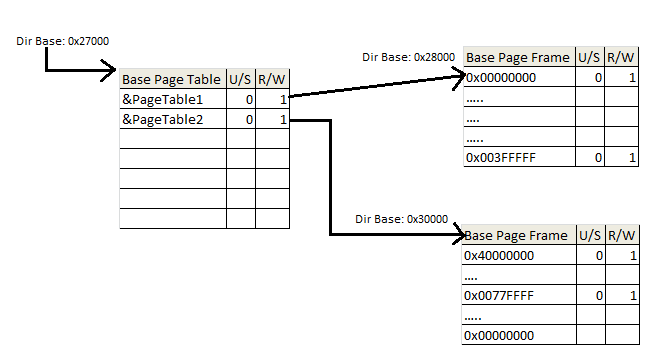
\includegraphics[scale=0.6]{imagenes/tablasDePaginasEj3.png}

\subsubsection{Activaci\'on de paginaci\'on}

Luego de armar el directorio de p\'aginas podemos habilitar la paginaci\'on. Para esto seguimo los siguientes pasos:
\begin{itemize}
 \item Cargar en CR3 la direccion al inicio del directorio de p\'aginas.
 \item Setear el bit mas significativo del registro CR0.
\end{itemize}





%%%%%%%%%%%%%%%%%%%%%%%%%%%%%%%%%%%%%%%%%%%%%%%%%%%%%%%%%%%%%%%%%%%%%%%%%%%%%%%
%% Conclusión                                                                %%
%%%%%%%%%%%%%%%%%%%%%%%%%%%%%%%%%%%%%%%%%%%%%%%%%%%%%%%%%%%%%%%%%%%%%%%%%%%%%%%

\newpage
\section{Conclusión}

Las instrucciones SIMD (Single Instruction Multiple Data) proveen al programador de una herramienta más efectiva para realizar el mismo conjunto de operaciones a una gran cantidad de datos.

La aplicación de filtros a imágenes era un ejemplo perfecto para probar su eficiencia.

Analizando los resultados de las implementaciones de los 3 filtros, podemos notar:

\begin{itemize}
\item Las operaciones básicas (padd, psub, pmul, pdiv, shifts, etc.) SIMD tienen un costo similar a sus correspondientes operaciones unitarias, pero generalmente requieren algún tipo de pre-proceso para poder trabajar con los 16 bytes (pack, unpack, shifts) en una sola iteración, por lo tanto, aunque más eficientes, no lo son en una relación directamente proporcional.
\item En el caso que sí hay una relación directamente proporcional es en el acceso a memoria.
\item Además, el acceso a memoria es, por lejos, la operación más costosa de las que implementamos en cada filtro.
\item Por consecuencia directa del ítem anterior, las llamadas a otras funciones (que a su vez, probablemente contengan variable locales) dentro de una iteración provocan estragos en la efectividad de las implementaciones en C.
\item Para poder aprovechar las instrucciones SIMD es un prerequisito que los datos estén contiguos en memoria.
\end{itemize}

Concluimos que, definitivamente, las instrucciones SIMD, cuando pueden aprovecharse, demuestran una gran eficiencia. Sin embargo, hay que tener algunas consideraciones:

Aunque las imágenes, video y sonido son los primeros candidatos a ser optimizados por paralelización, no todos los procesos pueden ser efectivos y se requiere un análisis profundo de los datos para ver si vale el esfuerzo.

Además, aunque se pueda lograr una gran optimización, no siempre es lo más importante. La optimización seguramente es indispensable en transmisiones de video en vivo, pero baja en importancia si tuviese que ser aplicado una sola vez en una aplicación tipo MS Paint.

Las desventajas que podrían opacar a la optimización son:

El código no es portable, únicamente funciona en procesadores que implementan el set de instrucciones AMD64, requiriendo reescrituras para otras plataformas. Sin embargo el código C debería funcionar perfectamente en IA-32, ARM y cualquier otro procesador que tenga un compilador de lenguaje C.

El código es mucho más largo y difícil de entender (por lo tanto mayor posibilidad de tener bugs) que en un lenguaje de más alto nivel como C. Y en pos de la optimización, se llegan a eliminar funciones (poniéndolas inline), lo que genera código repetido, largo y confuso.




\end{document}